\chapter{The LHC and CMS Experiment}

\clearpage
\section{The LHC}

The Large Hadron Collider (LHC) is the largest and most powerful particle accelerator in the world. The LHC was installed in an existing 26.7 km tunnel that was constructed for the LEP machine between 1984 and 1989. The LHC tunnel has 8 straight sections and 8 arcs, and is located between 45m and 170m below the surface. The LHC hosts 4 experiments currently: CMS (Point 5), ATLAS (Point 1), ALICE (Point 2) and LHCb (Point 8). The LHC can accelerate the proton beam to 7 TeV (running on 6.5 TeV during the LHC run2).

However, the LHC is not the only accelerator that boosts the proton to such a high energy. The LHC is the last and biggest accelerator in the whole chain. A simplified injection chain is illustrated by Fig~\ref{fig:c3lhclpsspslhc}. Hydrogen gas is injected into a metal cylinder, and then placed in a strong electrical field to strip the electron from hydrogen to obtain proton beam. The protons is accelerated to 90 keV with a DC voltage power supply. Then a Radio Frequency Quadrupole (QRF) focuses and boosts the protons beam to 750 keV. After that, the proton beam is injected into a linear accelerator (LINAC2) and accelerated to 50 MeV. The current LHC uses the LINAC2 as the source of protons. The LINAC2 will be replaced by LINAC4 with a negative hydrogen ion source, and a higher beam intensity and energy (160 MeV) in 2019-2020. 

\begin{figure}[htbp]
 \begin{center}
  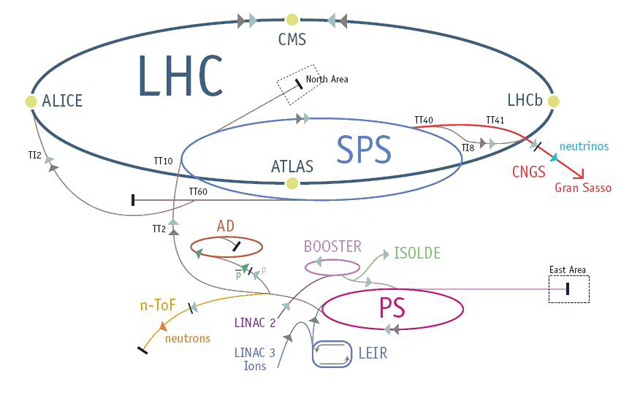
\includegraphics[width=0.8\textwidth]{figures/c3/c3_lhc_lpsspslhc.jpg}
 \end{center}
 \caption{The LHC full injection chain}
 \label{fig:c3lhclpsspslhc}
\end{figure}

The proton beam is boosted to 6.5 TeV with four circular accelerators from the linear accelerator. The first one in the chain is the proton synchrotron booster (PSB, Fig~\ref{fig:c3lhcpsb}), a four-ring slow-cycling synchrotron. The PSB was inserted in between the LINAC and proton synchrotron in 1972 to increase the beam intensity. The PSB increases the proton energy up to 1.4 GeV in 530 ms and then injects the beam to the proton synchrotron (PS). The protons are accelerated to 25 GeV inside the PS. PS forms the standard beam for the LHC injection. The super proton synchrotron (SPS) takes the beam from the PS and boosts it to 450 GeV in 4.3 seconds. And finally, the protons are injected into the LHC and are accelerated up to 6.5 TeV in 25 minutes during so-called beam ramp-up. 

\begin{figure}[htbp]
 \begin{center}
  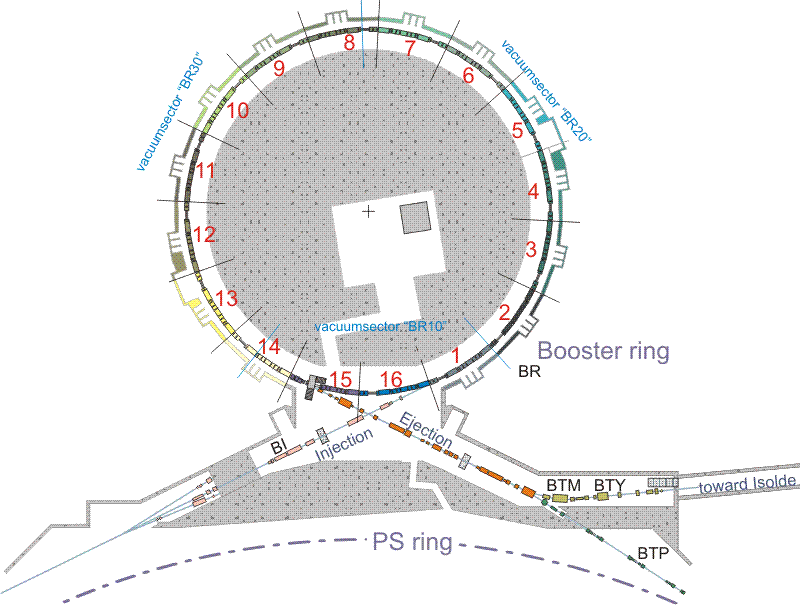
\includegraphics[width=0.8\textwidth]{figures/c3/c3_lhc_psb.png}
 \end{center}
 \caption{The PS layout}
 \label{fig:c3lhcpsb}
\end{figure}

We can perform a simple calculation to estimate how long it takes protons to travel from the LINAC2 until they have 450 GeV of energy in the SPS: 0.53+1.025+4.3=5.86 seconds. However, we also split one fill of the beam into several bunches and batches with certain time spacing to obtain a desired luminosity. Therefore, we have latency for different batch and the 5.86 seconds is just a lower limit for pre-LHC acceleration time. 

%The fill scheme before the LHC is relatively stable in the machine in the proton physics mode. The injection beam from the PSB to the PS contains 2 batches, 4 bunches for the first batch and 2 for the second. The first takes an additional 1200ms to be delivered. The proton beam will go through one triple split and two double splits. A 72 bunches beam will be formed after the splitting and delivered to SPS in a group of 4 72-bunch batches. The latencies are 10.8 seconds for the first batch, 7.2 for the second, 3.6 for the third and 0 for the fourth. Therefore, the maximum time from the LINAC2 to 450 GeV SPS is 0.53+1.2+1.025+10.8+4.3=17.86 seconds. 

The LHC fill scheme can be different for various purposes. A common fill scheme has 2808 bunches in the LHC ring. This fill scheme is illustrated in the Fig~\ref{fig:c3lhcfillscheme}. The SPS will have 12 injections to the LHC. The number of 72-bunch batches are in the pattern of 234 334 334 334. There are different luminosities for different fill schemes. In the detector operation, it is important to know the fill scheme and expected luminosity in advance to in order to design the trigger menu. 

\begin{figure}[htbp]
 \begin{center}
  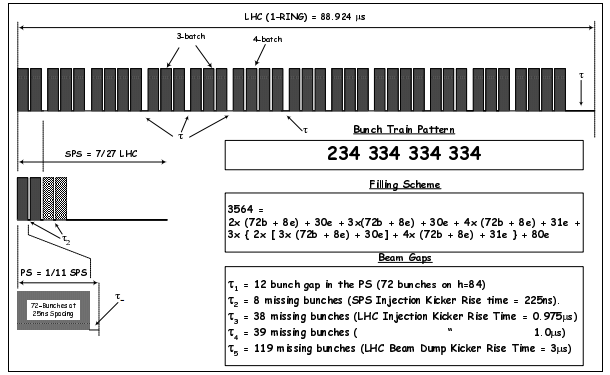
\includegraphics[width=0.8\textwidth]{figures/c3/c3_lhc_fillscheme.png}
 \end{center}
 \caption{Schematic of the Bunch Disposition around an LHC Ring for the 25 ns Filling Scheme}
 \label{fig:c3lhcfillscheme}
\end{figure}

\clearpage
\subsection{LHC: Machine layout and Performance}

The LHC is a nearly circular ring with 8 arcs and 8 straight sections (Fig~\ref{fig:c3lhclayout}). Each straight section is around 528 meters long and can host a detector system or beam related insertions. The general purposes experiments are located at opposite straight sections: ATLAS at point 1 and CMS at point 5. The ALICE experiment and the clockwise circulating beam (beam1) injection system are located at point 2, while the LHCb and counter clockwise circulating beam (beam2) injection system are at point 8. 

\begin{figure}[htbp]
 \begin{center}
  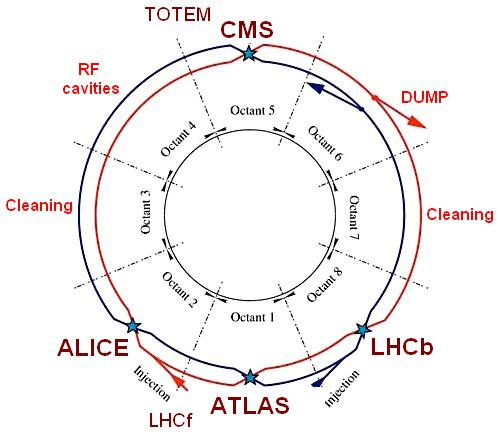
\includegraphics[width=0.8\textwidth]{figures/c3/c3_lhc_latticelayout.jpg}
 \end{center}
 \caption{The LHC layout}
 \label{fig:c3lhclayout}
\end{figure}

Two collimation systems\cite{Assmann:691766} are located at point 3 and point 7, respectively. The collimation system protects the machine against unavoidable regular or irregular beam loss. The collimator at point 3 is designed to clean beam transverse momentum dispersion and the one at point 7 is for beam betatron emission. The materials of the collimators are required to be extremely radiation hard because they are installed in the most active region of the LHC. 

The beam dump insertion is sits at the point 6. There are three steps to dump the beam: extraction, dilution and absorption. The magnet kicker will be turned on in 3000 ns, which is the gap reserved for each orbit cycling. Then the beam is kicked off by an angle of 0.27 mrad. The extracted beam will be swept in a quasi-circular orbit by two sets of deflecting dilution kickers. Finally, a 7m long segmented carbon cylinder will absorb the beam.

Point 4 is the only straight section that contains acceleration systems. Two radio frequency systems are installed for both beam1 and beam2. 

One of the main aims of the LHC is to reveal the physics beyond the standard model. The study of the rare events in the LHC requires both high beam energies and high beam intensities. The energy of the beam is limited by the machine geometry. The luminosity of the machine can be described by Eq~\ref{eq:c3lhclumi} with the Gaussian beam distribution. The $N_{b}$ term is the number of particles per bunch and $n_{b}$ is the number of bunches per beam. This indicates we can increase the luminosity with the optimization of fill scheme. The $f_{rev}$ term is the revolution frequency, $\gamma_{r}$ is the relativistic gamma factor, $\varepsilon_{n}$ is the normalized beam emittance and $\beta *$ is the impact parameter at the collision point. The F term is the geometric luminosity reduction factor due to the crossing angle at the interaction point. 

\begin{equation}
 L = \frac{N^{2}_{b}n_{b}f_{rev}\gamma_{r}}{4\pi \varepsilon_{n}\beta *}F \;
 \label{eq:c3lhclumi}
\end{equation}

The definition of F is given in Eq~\ref{eq:c3lhcgeof}. The $\theta_{c}$ term is the full crossing angle at the interaction point, the $\sigma_{z}$ is the RMS bunch length and $\sigma *$ is the transverse RMS beam size at the interaction point. The LHC experts are trying to reduce the crossing angle from 370 to 280 mrad, which will increase the peak luminosity by 15 percents. 
\begin{equation}
 F = (1+\frac{\theta_{c}\sigma_{z}}{2\sigma *})^{-1/2} \;
 \label{eq:c3lhcgeof}
\end{equation}

In the CMS and ATLAS experiments, the designed peak luminosity at the collision point is approximately $10^{34}cm^{-2}s^{-1}$. The LHC has achieved this goal in 2016 and now try to increase the luminosity through optimizations.

\clearpage
\subsection{LHC: From an operational point of view}

The LHC is an extremely complex machine and it is almost impossible to grasp every details. However, the LHC provides a summary of status for its operational activities, which are very useful in for detector operation.

\subsubsection{Acclerator Mode}

The accelerator mode indicator provides a summary of the status of the LHC machine. All the accelerator modes are listed in the Table~\ref{tab:c3lhcaccmode}. The accelerator modes can be divided into two groups by the presence or not of the beam. For example, ACCESS mode means the LHC group or at least one of the detector system groups needs access to the machine area, with the beams off, to investigate a problem. The beam must be dumped or already be off to allow this access period. Another example is the BEAM SETUP mode, which means the beam under preparation. The beam modes are described in the following section. The detector systems (e.g., CMS) make daily operational decisions depending on the accelerator modes and beam modes provided by the LHC.

\begin{table}[htbp]
\fontsize{10 pt}{1.2 em}
\selectfont
\begin{centering}
\caption{\label{tab:c3lhcaccmode} Acclerator Mode}
\hspace*{-4ex}
\begin{tabular}{|c|c|c|}
\hline
 Mode Name &  Description & Beam exist \\
\hline
 SHUTDOWN & \specialcell{Machine not running} & NO BEAM \\
\hline
 COOLDOWN & \specialcell{Machine comes back from shutdown,\\ cryogenics related activities going on} & NO BEAM \\
\hline
 MACHINE CHECKOUT & \specialcell{Checking out LHC subsystems} & NO BEAM \\
\hline
 ACCESS & \specialcell{Access going on} & NO BEAM \\
\hline
 MACHINE TEST & \specialcell{Operation tests without beam} & NO BEAM \\
\hline
 CALIBRATION & \specialcell{Power converter calibration} & NO BEAM \\
\hline
 WARM-UP & \specialcell{Sectors warm up for repair} & NO BEAM \\
\hline
 RECOVERY & \specialcell{Quench recovery} & NO BEAM \\
\hline
 SECTOR DEPENDENT & \specialcell{Sector activities going on} & NO BEAM \\
\hline
 BEAM SETUP & \specialcell{Machine setup with 1 or 2 beams,\\ usually a signal of next \\ physics fill when taking data} & BEAM \\
\hline
 PROTON PHYSICS & \specialcell{Beam on for proton physics} & BEAM \\
\hline
 ION PHYSICS & \specialcell{Beam on for ion physics} & BEAM \\
\hline
 TOTEM PHYSICS & \specialcell{Beam on for TOTEM physics} & BEAM \\
\hline
 MACHINE DEVELOPMETN & \specialcell{Beam on machine development} & BEAM \\
\hline
\end{tabular}
\par\end{centering}
\end{table}

\subsubsection{Beam Mode}
The beam modes are shown in the Table~\ref{tab:c3lhcbeammode}. The beam modes describe standard injection procedures and accidental abort issues of the two beams in the LHC. A standard successful injection for physics should have the following beam modes in sequence during BEAM SETUP accelerator mode:

\begin{itemize}
\item BEAM SETUP: The SPS is injecting beam bunches into the transfer line. The beam is not circulating yet in the LHC.
\item INJECTION PROBE BEAM: A test beam with relatively small intensity is being injected into the LHC from the transfer line. Although we have machine protection system to shield the LHC from the beam, we still need to make sure the system is safe for beam circulation.
\item INJECTION SETUP BEAM and INJECTION PHYSICS BEAM: The LHC is measuring the beam properties. Then a full intensity beam will be injected for physics data taking.
\item PRERAMP and RAMP: The LHC is ramping up the beam energy up with the radio frequency system.
\item FLAT TOP and SQUEEZE: The LHC is checking the system. Then the beam will be focused to reduce the impact parameter.
\item ADJUST and STABLE BEAM: The LHC is adjusting the beams before collision. Then we can begin to enjoy the data run.
\end{itemize}

\begin{table}[htbp]
\fontsize{10 pt}{1.2 em}
\selectfont
\begin{centering}
\caption{\label{tab:c3lhcbeammode} Beam Mode}
\hspace*{-4ex}
\begin{tabular}{|c|c|c|}
\hline
 Mode Name &  Description \\
\hline
 SETUP & \specialcell{Beam in transferline, but not in the ring} \\
\hline
 ABORT & \specialcell{Recovery mode following beam drop} \\
\hline
 INJECTION PROBE BEAM & \specialcell{Ring is injected with test beam for safe circulating} \\
\hline
 INJECTION SETUP BEAM & \specialcell{Beam measurement going on after probe beam\\ but before injection physics beam} \\
\hline
 INJECTION PHYSICS BEAM & \specialcell{Beam for physics is injected in the ring} \\
\hline
 PRERAMP & \specialcell{Injection done, prepare for ramp} \\
\hline
 RAMP & \specialcell{Ramp up the beam energy} \\
\hline
 FLAT TOP & \specialcell{Ramp done, pre-squeeze checks} \\
\hline
 SQUEEZE & \specialcell{Squeezing the beam size} \\
\hline
 ADJUST & \specialcell{Preparing for collision or after collision} \\
\hline
 STABLE BEAMS & \specialcell{Stable collision, detector should taking data} \\
\hline
 UNSTABLE BEAMS & \specialcell{Unstable beam because of sudden beam degradation} \\
\hline
 BEAM DUMP WARNING & \specialcell{Beam dump warning in case of emergency beam dump} \\
\hline
 BEAM DUMP & \specialcell{End of physics collision} \\
\hline
 RAMP DOWN & \specialcell{Ramp down beam energy after programmed dump} \\
\hline
 CYCLING & \specialcell{Pre-cycle before injection\\ following access, recovery, etc} \\
\hline
 NO BEAM  & \specialcell{No beams exist} \\
\hline
\end{tabular}
\par\end{centering}
\end{table}

The beam modes are used to estimate the time remaining before the beginning of the subsequent data run. For example, CMS requires all the subsystem to be ready for data taking when the LHC declares injection physics beam. Some of the subsystems need to do the alignment or calibration during this period. The time estimates allowed by using the LHC beam status is important for smooth data taking.

\clearpage
\section{The CMS Experiment}

The CMS Experiment is a particle physics experiment based on the CMS detector system at the LHC. It consists of the CMS detector system and event reconstruction, supported by the detector operation team, the computing/data storage team and , the software and event reconstuction team, the detector performance groups (DPGs), the physics objects groups (POGs), the phyiscs analysis groups (PAGs), the Publications Committee, the Conference Committee, the Authorship Committee, the spokesperson and deputies, and many other people.  In total, there are around 2500 individuals listed on a typical physics publication, and around 1000 more who contribute to the operation of the experiment.

\clearpage
\subsection{CMS Detector System}

The Compact Muon Solenoid (CMS) is one of the general-purpose detector system at the LHC. To fullfill its "general-purpose", the CMS is designed as a combination of several subsystems: Sillicon Pixels and Strips for tracking information, Electromagnetic and Hadron Calorimeters for "light" particle energy deposition and drift tubes and cathode strip/resisstive plate chambers for muon detection. The locations of these subdectors in the CMS are not random: The sillicon tracking subsystems are innermost to the collision point. The calorimeters come after the sillicon subdetectors, because the calorimeter absorb all SM particles except for muons and neutrinos. Finally the muon system is in the outermost layer. To obtain high performance, CMS is immersed in a 4-T magnetic field, which is provided by a superconducting solenoid ("S" in CMS). The magnet contributes a large fraction of the CMS total weight: 12500 tons out of 14000. However, compared with its heavy weight, the size of the CMS is relatively small: only 5000 $m^{3}$. In comparison, the ATLAS detector weighs 7000 tons and encompasses a volume of 22500 $m^{3}$. This explains the name "Compact" placed in front of "Muon Solenoid" since its density is nearly to 3000 $kg/m^{3}$.

\subsubsection{Inner Tracking system}

As indicated by the name --- inner tracking system, there are two main characteristics of this CMS sub-detector: it is the closest sub-detector to the LHC beam and its purpose is to reconstruct the trajectories of charged particles ("tracks") that traverse it. The main challenge is a consequence of the first feature: the inner tracking systems have to be radiation hard during the relatively long lifetime. Moreover, since the LHC has high intensity and a small time between bunch crossings (25 nano seconds), we also need the inner tracking systems to have a fine granularity and fast response. The silicon based technology detector is the best option to satisfy these requirements. On the other hand, the second feature actually comes from the physics requirement. We need to reconstruct the tracks of charged particles and secondary vertices in the event from the three dimensional hits. The track information is not only used in the charged particle reconstruction, but also applied in the particle flow algorithm\cite{CMS-PAS-PFT-09-001} as a basis of all physics object reconstruction in CMS. The secondary vertices are also important in the heavy flavor object reconstruction, and new-physics search of long-lived particles. 

As a result of budget-performance balance, the CMS inner tracking systems are designed as a combination of two sub-systems: the silicon pixel detector and the silicon strip detector. A schematic drawing of the CMS tracking system is shown in the Fig~\ref{fig:c3cms2dtracker}. More details are given in the following sections. 

\begin{figure}[htbp]
 \begin{center}
  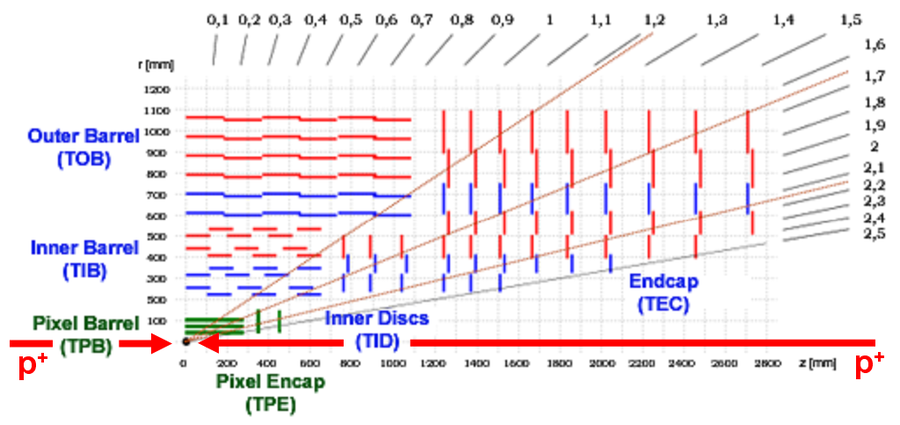
\includegraphics[width=0.8\textwidth]{figures/c3/c3_cms_2dtracker.png}
 \end{center}
 \caption{Two dimensional CMS inner tracking system layout, phase 0}
 \label{fig:c3cms2dtracker}
\end{figure}

\paragraph{Silicon Pixels}
The pixel system is the part of inner tracking system that is closest to the collision point. It provides a precise measurement of the tracking and therefore makes a major contribution to the secondary vertex reconstruction. The pixel cells are distributed with a size of 100 $\mu m$ $\times$ 150 $\mu m$ in three-dimensional space, which allows a 3D reconstruction method for the secondary vertex. The signals are read by sensors and packed by readout chip. Then the signal is delivered to the frondend driver through the analog chain once a positive bit is received from L1 trigger.

CMS detector system has three phases for different stages of the LHC. Phase 0 CMS is the baseline detectors for the LHC with 7 or 8 TeV and integrated luminosity around 25 $fb^{-1}$. Phase 1 CMS is the first detector upgrades for 13 or 14 TeV and integrated luminosity around 300 $fb^{-1}$. Phase 2 CMS is the major upgrade for high-lumi LHC (HL-LHC) with 3000 $fb^{-1}$. The phase 0 pixel detector contains three barrel layers (BPix) and two endcap disks (FPix), which covers a pseudorapidity range $-2.5<\eta<2.5$. The pseudorapidity $\eta$ is a spatial coordinate describing the angle angle of a particle relative to beam axis. It is defined as $\eta = -ln[tan(\frac{\theta}{2})]$, where $\theta$ is the angle between the particle three-momentum and beam direction. In the phase 1 upgrade\cite{Klein:2140071}, because of radiation damage, all layers and disks were replaced with new ones, and an additional layer was added both in the barrel region and in both endcap regions.

%One special design of the pixel detector is the blade that module mounted are rotated by 20 degrees in a turbine geometry. Such an arrangement enhanced the charge sharing effects\cite{Giurgiu:2008ir} between the nearby pixels. The space resolution can be improved to 15 $\mu m$ by the using the "charge sharing" effect in pixels. CMS take advantage of this effect with the analog readout of the collected charges by readout pixels in-group with readout chips. 

\paragraph{Silicon Strips}

The particles pass through ten layers of silicon strip detectors after the pixels. The silicon strip tracker is composed of 15148 detector modules. Each module carries either one 320 $\mu m$ or two 500 $\mu m$ silicon sensors from a total of 24244 sensors. The signal from a sensor is amplified, shaped and stored by a custom integrated circuit. Once a positive L1 trigger decision is received, the analog signal is multiplexed and transmitted via an optical link to the front end driver, then digitalized. 

The inner strip detector contains 4 barrel layers (TIB) and 3 endcap disks (TID) on each side. The outer strip detector has 6 barrel layers (TOB, 2 double-sided, 4 single-sided) and the endcap strip has 9 disks (TEC) on each side.

A laser alignment system\cite{Sirunyan:2017rbc} is used to monitor the stability and the alignment of the strip detector mechanical structure. An infrared laser light is delivered directly to the sensor on the 434 silicon modules (3\%) to trigger a signal pulse. The alignment data can be taken during commissioning, an inter-fill period or in the orbit gap with stable beams. The pixel detector is aligned with strip detector using the reconstructed tracks, and therefore the strip alignment is the only online and direct alignment needed for the inner tracking system. 

\subsubsection{Calorimeters}
\paragraph{Electromagnetic Calorimeter}
The CMS electromagnetic calorimeter (ECAL) is a hermetic homogeneous calorimeter made of lead tungstate ($PbWO_{4}$) crystals. Lead tungstate is an appropriate choice for the ECAL because the crystal is both radiation hard and has a rapid response (same level as the LHC bunch crossing). In total 61200 lead tungstate crystals are installed in the ECAL barrel region while 7324 are installed in each endcap. Lead tungstate emits 80\% of the light in 25 ns once an electron (or photon) strikes on the crystal.

A photon detector is needed to collect the light yield from crystals. As for the crystal, the photon detector needs to be both radiation tolerant and fast. To satisfy these requirements, avalanche photodiodes (APD) are installed in barrel and the vacuum phototriodes in the endcap. All the photon detectors have been tested in a harsh environment (high radiation plus 4T magnet field) before actually being installed. The light yield from the crystal is weak, so it needs to be amplified with a photomultiplier. Multi-gain pre-amplifiers (MGPA), an ASIC (Application-specific integrated circuit) specifically designed for ECAL, are installed to reshape and amplify the signal from photon detectors.

The amplified signals are integrated and digitized by on-detector front end electronics and then pass to the central data acquisition system from the off-detector back end electronics. The ECAL electronics, especially for the off-detector electronics, the ECAL are very similar to the phase 0 HCAL off-detector electronics. The HCAL electronics are discussed in the next section.

A last component of ECAL is the preshower system. The two photons from neutral pion decay are almost colinear when the pion energy is high. The main purpose of the preshower detector is to trigger an electromagnetic shower with high spatial resolution before the ECAL endcap. As a result, the almost collinear photons can be distinguished by the ECAL reconstruction algorithm. 

\paragraph{Hadron Calorimeter}

The CMS HCAL is a set of detectors that measure the energy of hadronic particles, i.e., particles composed of quarks and gluons. It contains four parts: Hadron Barrel (HB), Hadron Endcap (HE), Hadron Outer (HO) and Hadron Forward (HF). The overall geometry scheme is indicated in Fig~\ref{fig:c3cms2dhcal}. The CMS HCAL is a sampling calorimeter with brass absorber to trigger a shower and scintillator for the energy measurement. We take advantage of the dense absorber to fit the HCAL in the limited space inside the solenoid (Except for HO). However, the HCAL suffers from a relatively big fluctuation in energy deposit due to the invisible energy loss in the absorber and uncompensated design of the calorimeter. The following paragraphs provide more description of HB, HE, HO and HF.

\begin{figure}[htbp]
 \begin{center}
  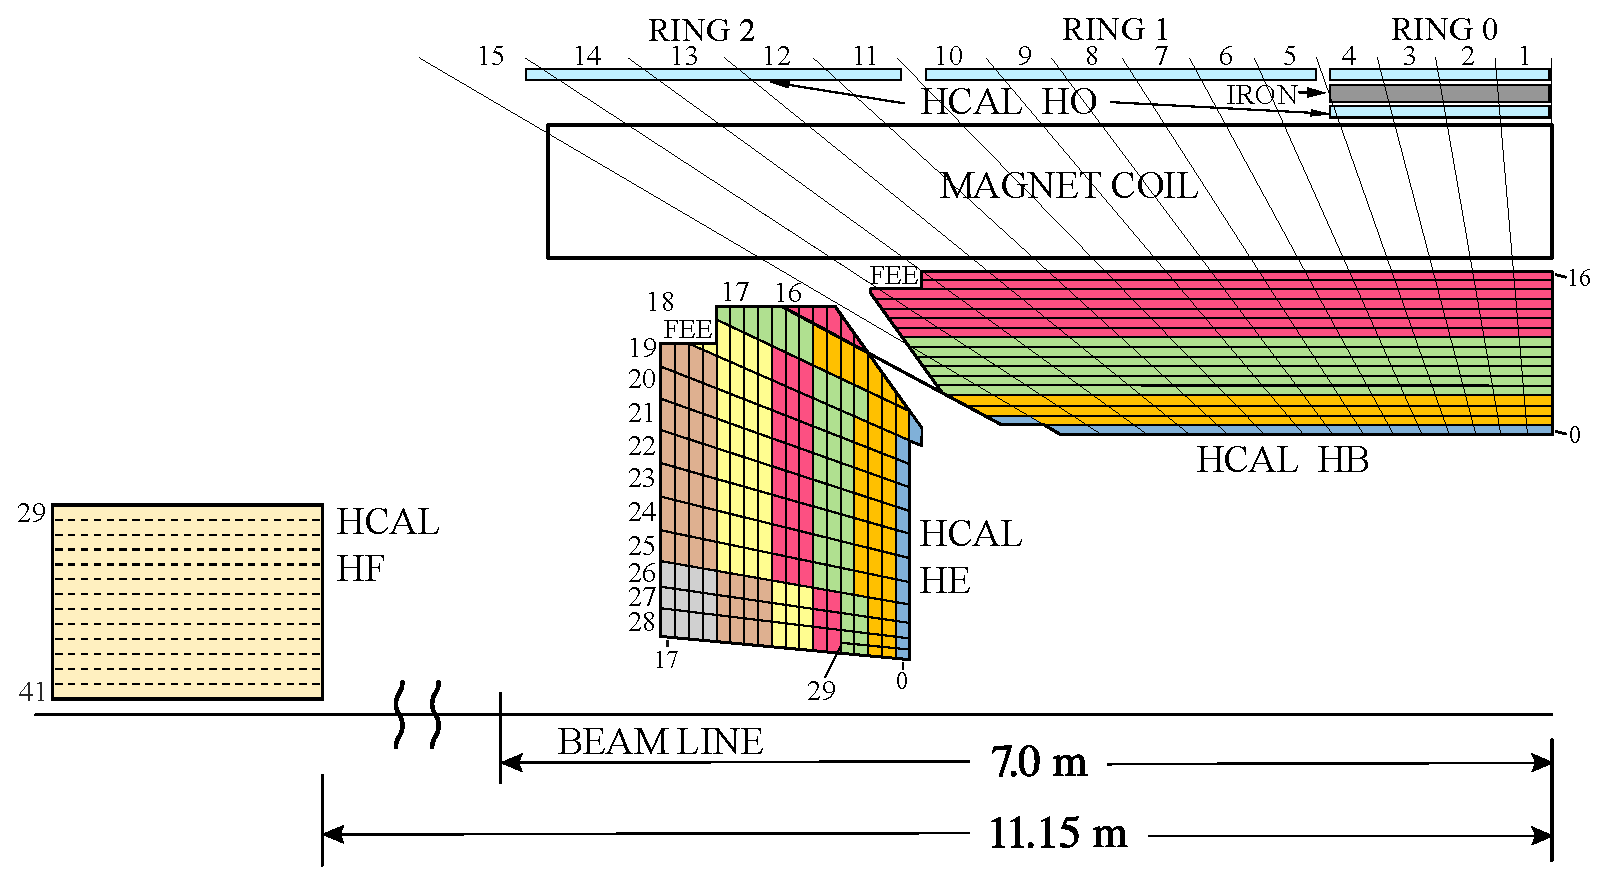
\includegraphics[width=0.8\textwidth]{figures/c3/c3_cms_2dhcal.pdf}
 \end{center}
 \caption{Phrase 1 HCAL tower segmentation in the r,z plane}
 \label{fig:c3cms2dhcal}
\end{figure}

The HB and HE are the major components of the HCAL. They are typical sampling calorimeters with brass from recycled Russia naval shell casings and scintillator for ~ 70000 tiles. Lights from the scintillators is collected and amplified by hybrid photodiodes (HPDs) in phase 0 HCAL. The HPDs will be replaced with Silicon photomultipliers (SiPMs) since the SiPMs are less noisy and more stable in heavy radiated area. 

After the photon detectors, the analog signal is delivered to the FrontEnd electronics. The charge pulse will be integrated and digitized on the charge integrator and encoder (QIE). In the phase 1 upgrade, we will replace the QIE8 with QIE11 for all frontend readout modules in HE. The QIE11 have a much better time resolution, which is on the level of 0.5 ns. 

After the FrontEnd, the digitalized signal is delivered from the commission cavern to the service cavern through a long bonded fibers bundle. The backend electronics located in the service cavern receives those signals, generates the trigger primitives and delivers the signals to the central DAQ link. The HCAL backend electronics were upgraded from VME to uTCA on HB and HE since 2015-2016 year-end technical stop (YETS)\cite{CMS:2012tda}. 

However, due to the limitations of the "compact" cavern, the EB and HB cannot provide complete containment for the hadronic showers. The HO is inserted just between the solenoid and muon system to ensure adequate sampling depth in the barrel region. The solenoid coil is used as the absorber for HO, which measures the shower deposit after HB. 

The HO detector construction is the same as the phase 0 HB and HE, except for the photon detectors. The HO has the SiPMs instead of HPDs since the LHC long shut down 1. The SiPMs have proved to be very reliable in the current operation except for a small leakage current drift monitoring issue at the beginning of LHC Run 2. 

The last component of HCAL is the Forward calorimeter (HF). The calorimeter material is severely challenged by the extremely high radiation environment. Therefore, quartz fibers are used as the active medium for HF. When a shower occurs, Cherenkov light is emitted in the quartz fiber and transported to the photomultiplier tubes (PMT). The HF also provides input to the CMS luminosity measurement. 

In summary, there are four subdetectors in HCAL: HB, HE, HO and HF. There are 9216 readout channels for HB, 6912 for HE, 2376 for HO and 3456 for HF in the HCAL phase 1 scheme. The backend electronics coordinates are compressed into the RAW event data after the event builder in the HLT. On one hand, the offline reconstruction software and online data quality monitor need to know the detector geometry coordinates to show the digitalized output in the physical space. We need to build a database object to map the backend coordinates and detector coordinates. On the other hand, the backend electronics are not connected directly to the HCAL tiles: we still have photomultiplier and frontend electronics in between. And HCAL has several different upgrade projects for different parts of different sub detectors during the LHC Run 2. Therefore, we need a dynamic map, which reflects the real connections among all HCAL components. This map is called HCAL logical Map. The logical map starts with frontend coordinates, maps upwards to the photomultipliers, and then detector tiles, and downwards to the backend coordinates and trigger primitive channels. We avoid re-designing everything after the each upgrade with this dynamic structure of the map. 

To build a robust HCAL logical map, we need inputs from experts in different fields. For example, we need to follow a special symmetric design in the frontend to backend optical patch. This symmetry is highly dependent on the firmware design. Although nowadays FPGA (Field Programmable Gate Array) can be programmed with less restriction, we still need to keep the algorithm maintainable. We also plot the backend and detector coordinates respectively in frontend coordinates in order to check the symmetry in mapping (Fig~\ref{fig:c3cmshcalhelmapfebe} and Fig~\ref{fig:c3cmshcalhelmapfegeo}).

\begin{figure}[htbp]
 \begin{center}
  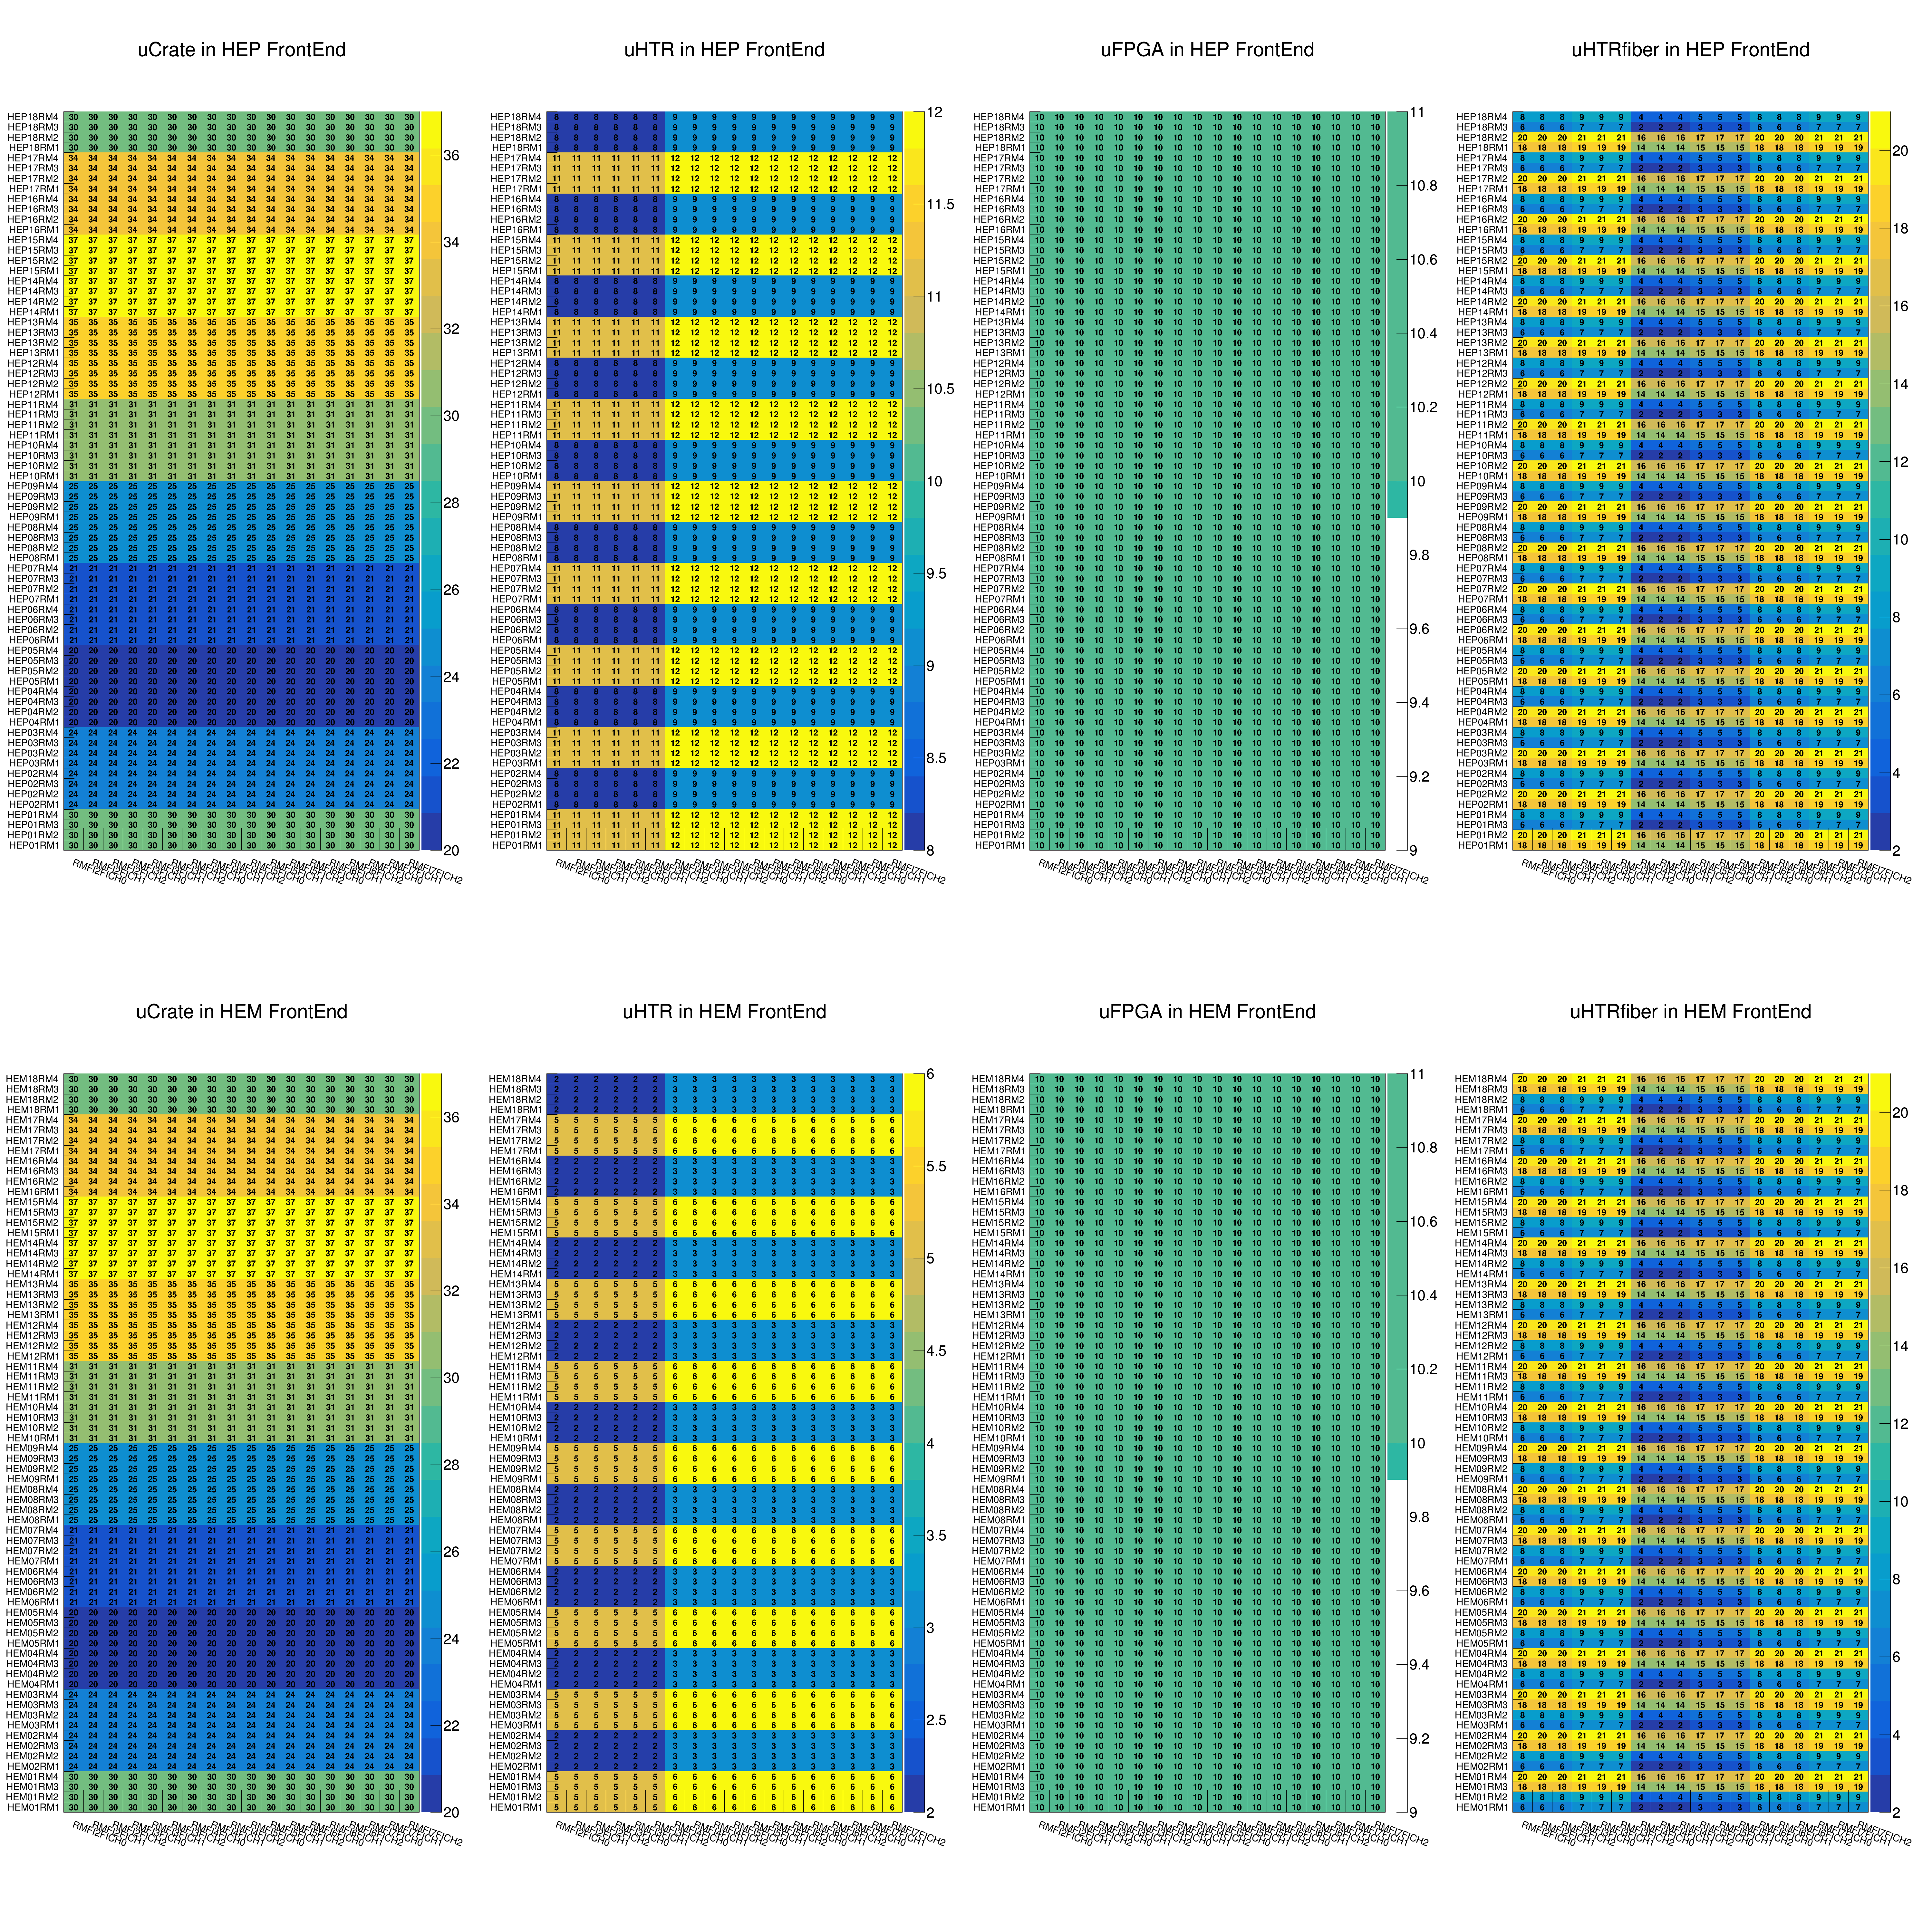
\includegraphics[width=0.8\textwidth]{figures/c3/c3_cms_hcalhelmapfebe.png}
 \end{center}
 \caption{Backend coordinates in Frontend coordinates, HCAL endcap phase 1 backend plus phase 0 frontend in 2016 operation}
 \label{fig:c3cmshcalhelmapfebe}
\end{figure}

\begin{figure}[htbp]
 \begin{center}
  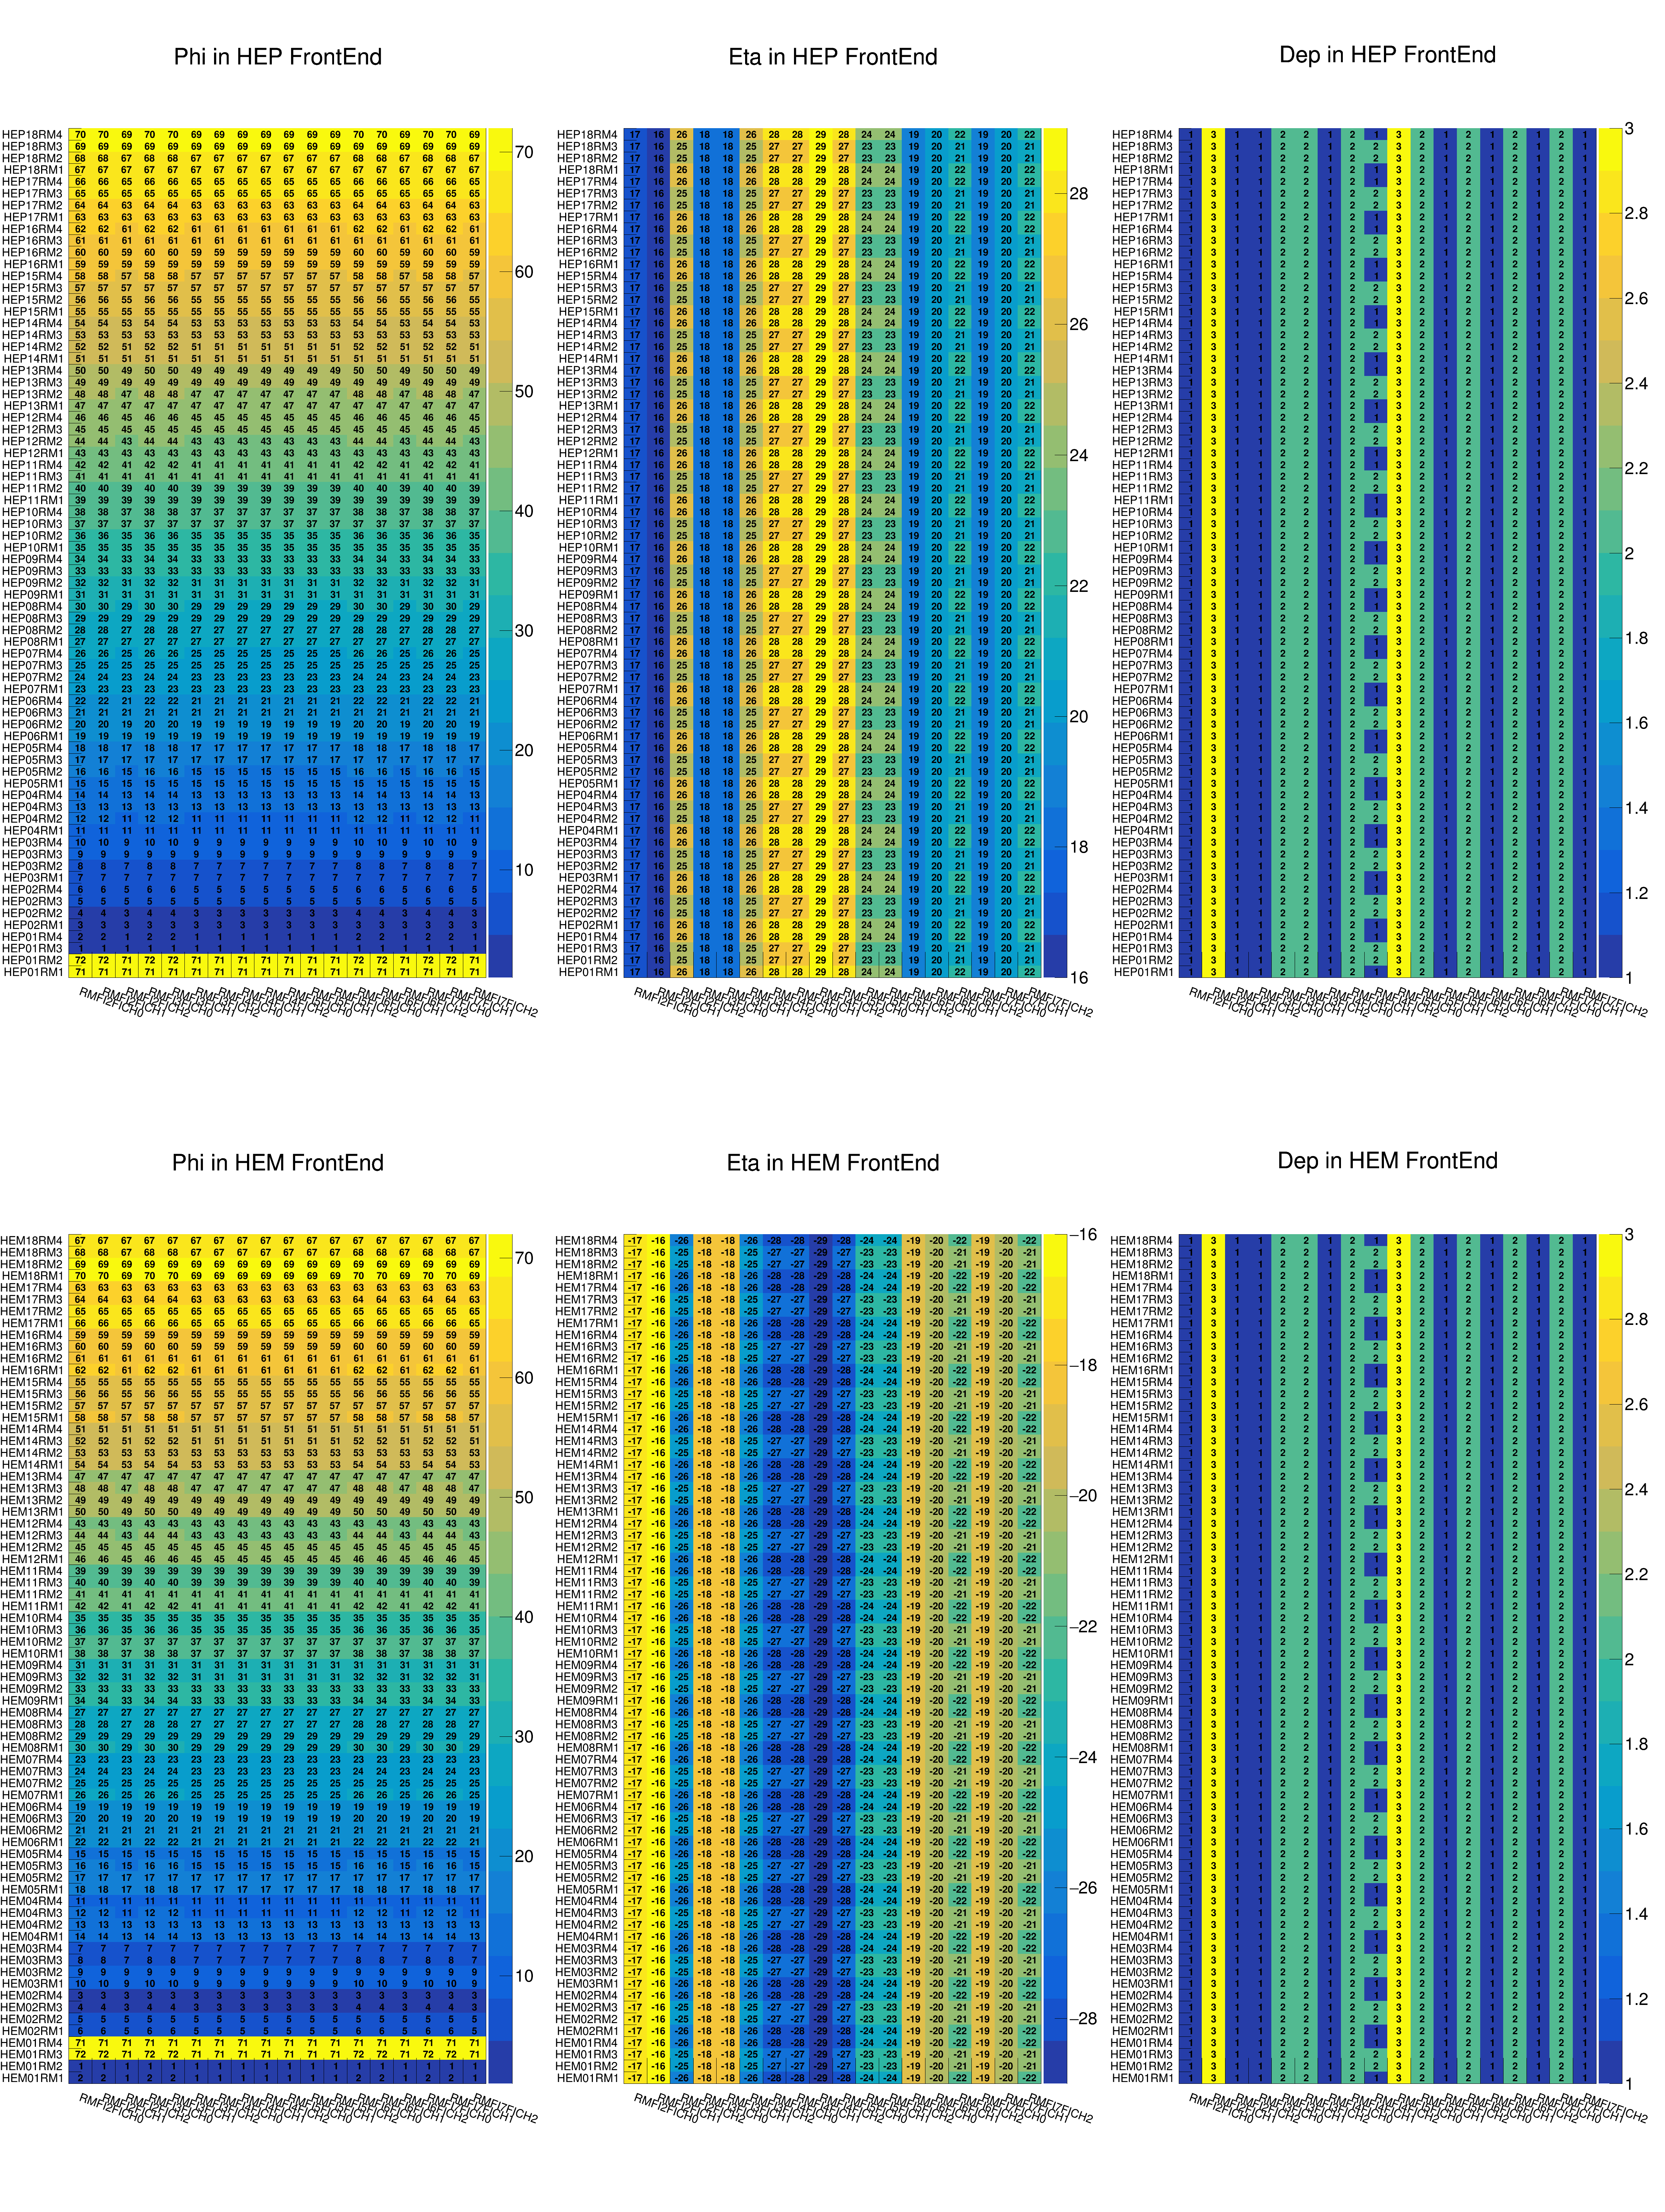
\includegraphics[width=0.8\textwidth]{figures/c3/c3_cms_hcalhelmapfegeo.png}
 \end{center}
 \caption{Detector coordinates in Frontend coordinates, HCAL endcap phase 1 backend plus phase 0 frontend in 2016 operation}
 \label{fig:c3cmshcalhelmapfegeo}
\end{figure}


Subsets of the HCAL logical map are critical in the HCAL software. One of the most important applications is the electronics map (EMap). The HCAL electronics map is a subset of logical map that contains backend coordinates and detector coordinates. As was mentioned, the reconstruction software needs the EMap database to obtain the detector coordinates from the backend coordinates. This is a necessary step in the RAW to DIGI reconstruction and in DIGI to RAW in MC simulation. Another application is the QIE calibration table. In the DIGI to RECO step, we need to translate from ADC (Analog Digital count) to the fC with the piecewise linear QIE gain function. This map is produced from the logical map. The robustness of the logical map is critical for the HCAL offline reconstruction. 

\subsubsection{Muon Detectors}

The importance of the Muon detectors is implied by the experiment’s middle name ("M" in CMS). The CMS muon detectors provide measurements of muon track coordinates. The measurement of muons is important in both in standard model physics (e.g. Higgs to ZZ) and in new physics search (e.g. searches for supersymmetric particles that can decay to leptons). Moreover, the muon system provides a muon-related level-1 trigger that is used to reduce the data rate.

The CMS muon detectors consist of three sub-detectors: Drift tubes in the barrel region, cathode strip chambers in the endcap and resistive plate chambers in both the barrel and endcap. A layout of CMS muon detectors is shown in Fig~\ref{fig:c3cms2dmuondets}. More details are given in the following sections. 

\begin{figure}[htbp]
 \begin{center}
  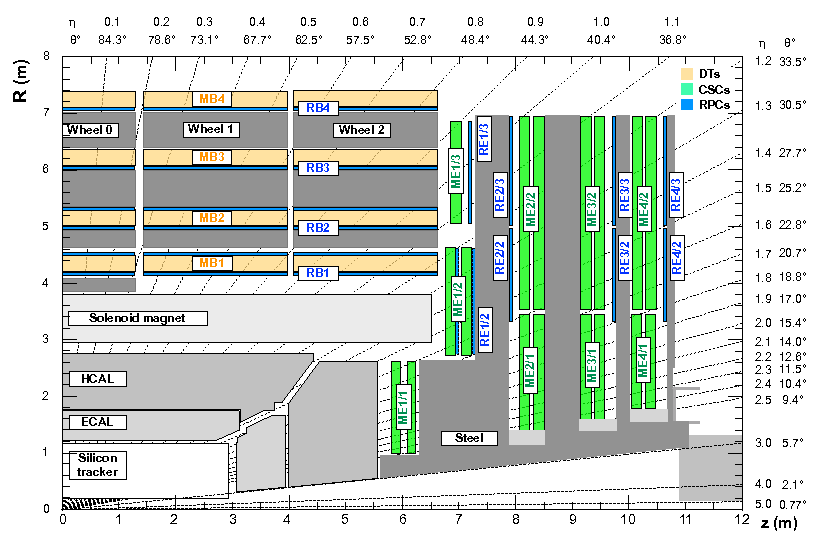
\includegraphics[width=0.8\textwidth]{figures/c3/c3_cms_2dmuondets.png}
 \end{center}
 \caption{Two dimensional CMS inner tracking system layout, phase 0}
 \label{fig:c3cms2dmuondets}
\end{figure}

\paragraph{Drift Tubes}
The drift tubes (DT) are the part of CMS muon detectors that measure the muon tracks in the barrel region. The basic unit of the drift tubes is the drift cell. A drift cell is a 42mm-wide tube contains a thin conductive wire at high positive voltage within a gas volume. The muon knocks electron off the atom of the gas when it travels. The muon tracks can be reconstructed by measuring the drift time for different cells. 

Like the HCAL outer detector, the Drift tubes contain 5 wheels along the z-axis, 4 stations for each wheel, labeled as MB1, MB2, MB3 and MB4. The three inner stations have 60 drift chambers each and the outer chamber has 70. A drift chamber consists of 2 or 3 super layers, each made of by 4 layers of drift cells staggered by half of cell. This honeycomb geometry gives an excellent time-tagging capability, with a time resolution of a few nanoseconds. The full DT provides the pseudo-rapidity coverage $0<|\eta|<1.2$.

\paragraph{Cathode Strip Chambers}
The cathode strip chambers (CSC) are the CMS muon detectors located in the endcap region. The CSC is also a type of wire chamber, but differently from the DT, the CSC measures the location (to be specific, phi coordinates) instead of drift time. The CSC consists of arrays of positively charged anode wires crossed with negatively charged copper cathode strip within a gas volume. The muon knocks the electron off from the gas atom. Then the electron moves to the anode wire to create an avalanche. Positive ions also move to the cathode and trigger a charged pulse.

The CMS endcap muon system consists of 468 cathode strip chambers in the following arrangement: 72 ME1/1, 72 ME1/2, 72 ME1/3, 36 ME2/1, 72 ME2/2, 36 ME3/1, 72 ME3/2, and 36 ME4/1. The full CSC provides the pseudo-rapidity coverage $1.2<|\eta|<2.4$. 

The RPC is designed as a fast response provider to the trigger. However, for the endcap region, the CSCs by themselves are sufficient for the trigger requirements for the current instantaneous luminosity of the LHC. Moreover, the CSCs have a better spatial resolution and a larger pseudo-rapidity coverage, providing better precision for the measurements of endcap muons.

\paragraph{Resistive Plate Chambers}
Resistive plate chambers (RPC) are fast gaseous detectors that provide a muon trigger system in parallel with the DT and CSC. The RPC consists of a two high resistively plastic parallel plates with gas between them. One of the plates is a positively charged anode and the other is a negatively charged cathode. Like the CSC, an electron of a gas molecule will be knocked off when a muon passes through, and trigger an avalanche. The pattern of hits on the cathodes provides a quick measurement of the muon momentum, which is passed to the trigger for decision-making. In the CMS RPC, the double-gap modules are used instead of the single-gap modules. This allows a lower bias voltage for each single-gap and higher detector efficiency. The RPC has both good spatial resolution and time resolution (one nanosecond). 

The CMS RPCs are distributed in both the barrel and endcap regions. There are 96 RPCs each in wheel in the barrel region. More details on the distribution are given in Table~\ref{tab:c3cmsrpc}. In the endcap region, there are 3 RPC stations in the phase 0 design. In order to keep the high muon reconstruction efficiency with Run 2 condition, the fourth disk was installed during the long shutdown 1 as part of the phase 1 upgrade. The full RPC has the same pseudorapidity coverage as the DT in barrel, and a smaller coverage ($1.2<|\eta|<2.1$) than the CSC in the endcap.

\begin{table}[htbp]
\fontsize{10 pt}{1.2 em}
\selectfont
\begin{centering}
\caption{\label{tab:c3cmsrpc} Numbers of RPCs for different wheels}
\hspace*{-4ex}
\begin{tabular}{|c|c|c|c|c|c|c|}
\hline
 RPC &  W+2 & W+1 & W0 & W-1 & W-2 & Total \\
\hline
 RB1(in) & 12 & 12 & 12 & 12 & 12 & 60 \\
\hline
 RB1(out) & 12 & 12 & 12 & 12 & 12 & 60 \\
\hline
 RB2/2(in) & 12 & - & - & - & 12 & 24 \\
\hline
 RB2/2(out) & - & 12 & 12 & 12 & - & 36 \\
\hline
 RB2/3(in) & - & 12 & 12 & 12 & - & 36 \\
\hline
 RB2/3(out) & 12 & - & - & - & 12 & 24 \\
\hline
 RB3 & 24 & 24 & 24 & 24 & 24 & 120 \\
\hline
 RB4 & 24 & 24 & 24 & 24 & 24 & 120 \\
\hline
 Total & 96 & 96 & 96 & 96 & 96 & 480 \\
\hline
\end{tabular}
\par\end{centering}
\end{table}

\subsubsection{Trigger system}

The LHC has a bunch crossing every 25 ns, which means 40 MHz in data rate. It is impossible for the data acquisition and storage system to deal with all of them and it is not necessary either, since not all the events are interesting for physics analysis. Therefore, we need a system to reduce the data rate and select the events that we are interested in. The system is called trigger system - - - only triggered data will be read and stored from the LHC collision. 

The CMS trigger system is a 2-level trigger system: the FPGA based L1T (Level 1 trigger) and PCs farm based HLT (High level trigger). In the old days (e.g. Tevatron, CDF trigger) there was a custom hardware L2T layer between the L1T and HLT to ease the computing speed gap. However, with improvement to the computing power of the PCs farms, we can avoid the additional L2T. This gives a more robust system with a less complicated structure. 

The CMS L1T system receives part of its information from the sub detectors and performs a rough reconstruction of physics object at the FPGA level. The data rate is reduced from 40 MHz to 100 kHz (85 kHz to 90 kHZ in real operation, mainly limited by the data acquisition system) after the L1T. The CMS L1T has been upgraded (Phase 1) during the 2015-2016 YETS and 2016-2017 EYETS to account for the large increase in the LHC beam intensity in Run 2. The scheme for the phase 1 L1T is shown in Fig~\ref{fig:c3cmsl1scheme}. The calorimeters send the trigger primitive to the calo trigger layer from where the signals are sent to the global trigger. The muon system sends information to the global muon trigger from where they are sent to the global trigger. The L1A (level 1 acceptance) is generated and sent to the sub detectors through TCDS (timing, control and distribution system). The sub detectors send the information to data acquisition or keep on taking data for next bunch crossing based on the L1 decision. 

\begin{figure}[htbp]
 \begin{center}
  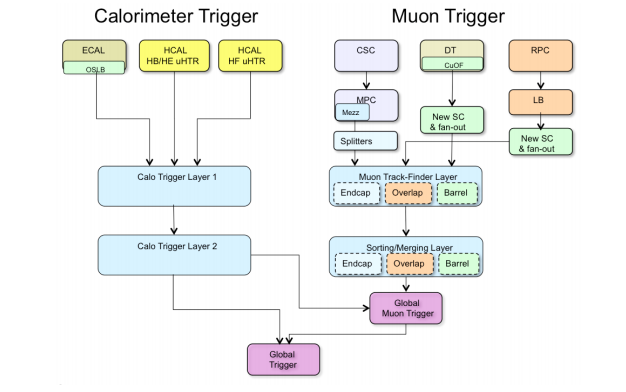
\includegraphics[width=0.8\textwidth]{figures/c3/c3_cms_l1scheme.png}
 \end{center}
 \caption{Dataflow for the overall phase 1 trigger system}
 \label{fig:c3cmsl1scheme}
\end{figure}

The CMS HLT system uses all the information from the detector readout and applies a simplified algorithm to reconstruct physics objects. Promptly reconstructed objects used in the high-level trigger menu for various physics purpose. However, just like the L1T, the HLT has bandwidth limitations. The data rate after the HLT is around 1000 Hz which is limited mainly by offline storage rather than online computing. HLT is the interface between physics analysis and online operation. On one side, each physics analysis group has a trigger contact person to collect the desired trigger menu from analyzers and make a proposal of a full menu set with rate estimation to the HLT that satisfies the data rate limit. On the other side, each HLT menu takes at least one L1 seed as a starting point of the high-level trigger.

The current (Phase 1) trigger system will be continue in operation until the end of LHC Run 3. However, there is a huge challenge on the trigger system with the following HL-LHC. The Track trigger will be necessary to maintain the current physics acceptance with the L1 rate around 1 MHz. 

\clearpage
\subsection{Event Reconstrunction}

The data from the central data acquisition system will be selected and built in the high-level trigger farm and then transferred to the primary computing grid at CERN (Tier-0). The data directly from the detector electronics is called DAQ-RAW, which is the input of the online HLT cluster. The data will be reformatted and filtered with high-level trigger in the cluster. The outcome data is called RAW. Comparing to the DAQ-RAW, the RAW contains the HLT information and ready for offline reconstruction after reformatting. 

Before entering the offline reconstruction chain, the data stream is filtered into different primary datasets (PD) for various purposes. Most of the categories are based on physics analysis and level 1 trigger. For example, in the all-hadronic SUSY search, the common PD for search region is HTMHT or MET. For the control region, we can select SingleElectron or SingleMuon PD. Then, the RAW with different PD streams will be delivered into the offline reconstruction system (CERN Tier-0 or any Tier-1, Fig~\ref{fig:c3cmstiers}). 

\begin{figure}[htbp]
 \begin{center}
  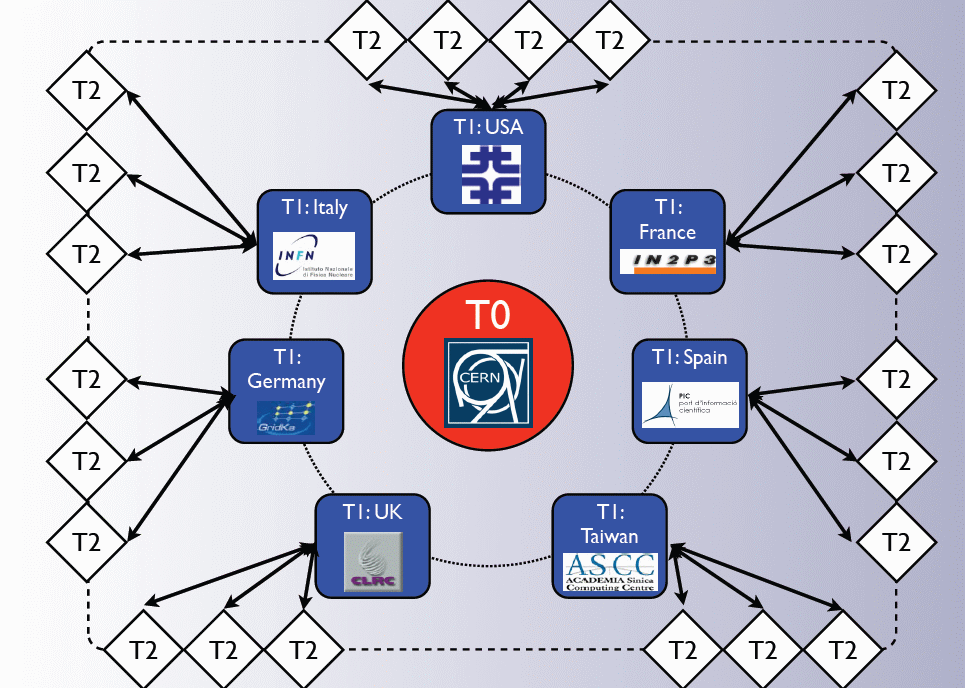
\includegraphics[width=0.8\textwidth]{figures/c3/c3_cms_tiers.png}
 \end{center}
 \caption{CMS offline computing structure}
 \label{fig:c3cmstiers}
\end{figure}

In the offline reconstruction, the RAW dataset will be unpacked from the electronics based digital counts to detector based digital hits. This is so called RAW to DIGI step in the reconstruction. After that, the DIGI will be converted to reconstructed hits with calibration information. This is called DIGI to RecHits step. The offline database are highly involved in these 2 steps, providing electronic-detector map, calibration table, pedestal subtraction, radiation damage correction, etc. Then, the physics objects will be generated with the reconstructed algorithm. The outcome dataset after the offline reconstruction is called RECO, which combines the RecHits and physics object information together. 

However, the size of the RECO dataset is about 1.3 MB per event. The further reduce of the data size is necessary for the physics analysis. Therefore, the information that not very commonly used for physics analysis is dropped to form a new data format: miniAOD. It contains the standard physics objects that used by most of the CMS physics analysis group. More details of those objects will be discussed in the following sections. 

\subsubsection{Tracks}

Tracks are detected by inner silicon detector signals in the CMS to form the basis of the event reconstruction. Track reconstruction serves the following purposes: 
\begin{itemize}
\item Vertex reconstruction: The vertexes in the proton-proton collision can be reconstructed from the gather point of tracks. However, there can be multiple vertexes in one event because the pile up effect. The vertex with the maximum sum of the square of the $p_{T}$ of all the associated tracks is identified as the primary vertex. We can also reconstruct the secondary vertex from the primary one. The secondary vertex information is useful in the b-jet identification.
\item Momentum measurement: The CMS inner silicon system has a high resolution in the track momentum measurement because of the strong magnetic field (3.8T). The jet $p_{T}$ measurement benefits a lot from the high precision track momentum with the particle flow algorithm. More details will be covered in the jet reconstruction section.
\item Particle identification: The charged can be identified with track information. For example, an electron candidate is found when the energy deposit in ECAL supercluster can be associated with track. Muon identification can also benefits from the inner track matching technique.
\end{itemize}

Given the importance of track reconstruction in physics, a reliable algorithm is required. The desirable algorithm must have a near 100\% efficiency in track reconstruction together with relatively small fake rate. The jet energy can be deadly mis-measured with an unidentified or fake track.
There are two steps in the track reconstruction: 
\begin{itemize}
\item Local reconstruction: the signals from the strip and pixel are clustered to evaluate the position and error matrices of hits.
\item Global reconstruction: Tracks are reconstructed with several iteration of the combinatorial track finder method\cite{Adam:2005cg}. Different seed will be used in different iteration to improve the tracking efficiency for various types of tracks.
\end{itemize}
The track finder algorithm is very powerful. It can even find the track with very low energy ($p_{T}<2 GeV$). Some of the low energy tracks have more number of hits than the number of detector layers, others tracks cannot reach to the preshower. Those tracks are kept in the data file for the low energy physics study at CMS. 

\subsubsection{Electrons}
The electron reconstruction in CMS relies on the information from inner tracker and ECAL. The track momentum can be measured with smaller uncertainty in the inner tracker system. On the opposite, the calorimeter has a better resolution for the high-energy object. Therefore, a mixture of "ECAL seed" and "tracker seed" algorithm is designed to optimize the electron identification in both high and low $p_{T}$ spectrum. 

The ECAL seed electron identification algorithm starts from the supercluster energy deposit in the ECAL. The supercluster is a 5 by 5 cluster combo in the ECAL. The initial energy and position in the supercluster will be used to estimate the electron trajectory in the first tracker layer. On the opposite, the tracker-based method begins with the tracks that are reconstructed by the general algorithm for charged particles. The tracks will be sent to a pre-selection and then matched to the ECAL supercluster. This mixture seed method has been validated with electron from W boson decay in 2010\cite{Khachatryan:2015hwa}. 

The electron identification group also provides several working points to satisfy the needs from various physics analysis. For example, we choose the "Veto" working point in the SUSY analysis described in this thesis. The "Veto" has the loosest identification criteria, which help us to reject leptonic decayed background to the most extent. 

\subsubsection{Jets and Particle Flow}

The jet is a collimated flux of stable hadrons that originate from quarks and gluons after fragmentation and hadronization. The jet algorithm is the approximate method to reverse the fragmentation and hadronization processes.  There are several different jet algorithm approaches. But the inputs of the jet algorithm are always the clustered energy deposits in 2-dimensional plane. 

There are two major requirements for the jet algorithm: collinear safe and infrared safe. The collinear safe means the results of the jet algorithm are invariant under collinear splitting of any input pixels. The infrared safety indicates that a soft emission will not change the results of jet algorithm. The infrared safety is requested not only from the soft emission QCD, but also from the collider point of view: the jet algorithm results should not change just because of a soft pile-up jet. 

The anti-$k_{T}$ algorithm\cite{Cacciari:2008gp} is the default jet algorithm for all the LHC experiments. The anti-$k_{T}$ algorithm is one of the sequential recombination algorithms. In this approach, we define a special distance of the two input observables in the Eq~\ref{eq:c3cmsantikt}:

\begin{equation}
 d_{ij} = min(k_{Ti}^{-2},k_{Tj}^{-2})\frac{(y_{i}-y_{j})^{2}+(\phi_{i}-\phi_{j})^{2}}{R^{2}} \;
 \label{eq:c3cmsantikt}
\end{equation}

Where $k_{Ti}$ means the energy (or any other response) of the ith input pixel. The numerator is the geometrical distance between the two objects. R is the cone size parameter in the algorithm. The CMS experiment now support R=0.4 for the normal jets and R=0.8 for the fat-jets, which is useful for the boost object. The special distance between the input pixel and beam is defined as: $d_{iB} = k_{Ti}^{-2}$.

The first step is to compute all the $d_{ij}$ and $d_{iB}$, and find the smallest one. Then iterate the following steps until all pixels are clustered into jet: 

\begin{itemize}
  \item If the smallest one is a $d_{ij}$, we combine the two pixels i and j. Then we recalculate the special distance as the input of next iteration.
  \item If the smallest one is a $d_{iB}$, we remove pixel i and call it a jet.
\end{itemize}

The anti-$k_{T}$ algorithm is obviously both collinear safety and infrared safety. A new collinear pixel means the geometrical distance is 0. Therefore the new pixel will be clustered first. A new soft pixel means the special distance will go to infinity. Therefore this new pixel will be clustered last or form a new zero jet. The jet results for the anti-$k_{T}$ algorithm remain unchanged for the both cases. 

However, there are other algorithms that are both collinear safety and infrared safety, like SiSCone\cite{Salam:2007xv} and $k_{T}$\cite{Cacciari:2005hq}. The jets from anti-$k_{T}$ algorithm always have a near-circle jet area\cite{Cacciari:2008gn}, which makes them easier to correct for the detector-related effects.

Now we have a reliable jet algorithm to combine the input pixels into jets. However, we can improve the performance by a more precise measurement on the energies of input pixels. In CMS experiment, we use particle flow (PF) algorithm\cite{CMS-PAS-PFT-09-001} to construct PF candidate as the input of CMS PF jets clustering. 

The particle flow (PF) is a stable particle reconstruction and identification algorithm that uses the information from all sub detectors in the detector system. The PF algorithm is important especially for CMS jet and missing transverse energy reconstruction due to the uncompensated nature of CMS HCAL. A jet usually has three components: charged hadron ($\pi^{+},\pi^{-}$, etc.), photon ($\pi^{0}$), and neutral hadron ($K_{L}$, etc.). The fractions of three components are listed in the Table~\ref{tab:c3cmsjetf}. The inner tracker can perform a more precise measurement of charged hadron fraction. The CMS ECAL also provides an excellent measurement on the photon energy. The remaining 10\% neutral hadron fraction will not give a huge uncertainty to the final measurement, on the average level. 

\begin{table}[htbp]
\fontsize{10 pt}{1.2 em}
\selectfont
\begin{centering}
\caption{\label{tab:c3cmsjetf} Average Jet components in GEANT4 Simulation}
\hspace*{-4ex}
\begin{tabular}{|c|c|c|c|}
\hline
Jet Constituent & Energy Fraction & Detection Instrument & Resolution \\
\hline
Charged Hadron  & 65\% & Inner Tracker & Negligible \\
\hline
Photon          & 25\% & ECAL &  $0.07^{2}E_{jet}$ \\
\hline
Neutral Hadron  & 10\% & ECAL and HCAL & $0.16^{2}E_{jet}$ \\
\hline
\end{tabular}
\par\end{centering}
\end{table}

The key part of the PF algorithm is the charged fraction linking between the tracker and calorimeter. First, we have tracks collection by the iterative track reconstruction method that described in previous section. Then, we will cluster the calorimeter to obtain an initial separation the photon, charged hadron and neutral hadron. Then a complicate linking algorithm\cite{CMS-PAS-PFT-09-001} will be applied to chain the objects from inner tracker and calorimeters up. 

The PF jets are still not the collection that we can directly use in the physics analysis. The PF jets energies still need to be corrected to match the energies of true particle jets. For the real data, there are three corrections need to be applied. The first one is the pile-up and noise correction. This correction is related to the real collider and detector effects and should be subtracted from the raw energy. The second one is the MC simulation correction. This is a pure evaluation on the reconstruction algorithm effect with MC samples. Finally, the jet energy will be corrected with di-jet data sample after the previous two corrections. More details of the jet energy corrections are described in\cite{1748-0221-6-11-P11002}. The jet energy corrections are applied in both data and MC in the physics analysis described in this thesis. 

\subsubsection{Missing Transverse Energy}

The missing transverse energy (\MET) is the imbalance in the transverse momentum of all visible particles. The \MET is an important variable in the R-parity conserved supersymmetry search since the lightest stable particles are heavy, stable in the physics model. The \MET is a powerful variable to suppress the standard model background in the search region. 
However, on the reconstruction side, the \MET is a high-level variable since all visible particles involved in the calculation. The unexpected effects from detectors and collider or issue in any objects reconstruction can give us the wrong \MET. Therefore, we need to establish robust \MET filters before we use the \MET, especially for the high \MET case. The source of the abnormal \MET event can be HCAL noise in HPD, beam halo, etc. 

After the filters, the \MET also need to be corrected, like jet energy correction. The most popular correction method is to propagate the jet energy correction to \MET (so called Type 1 correction). We apply the type 1 correction in this analysis. More details of the \MET filters and corrections are covered in\cite{CMS-PAS-JME-16-004}. 


\subsubsection{Muons}
The muon is a heavy particle that can penetrate the calorimeter and detector by the muon system outside the solenoid. The muon reconstruction has two traditional approaches: 

\begin{itemize}
	\item Global Muon reconstruction: The muon tracks are reconstructed first inside the muon system (DT, RPC, CSC) by a standalone method. Then, the muon standalone muon track will be matched with a tracker track by comparing the parameters of the two tracks. Finally, a global muon track will be derived from the hits of the two tracks by Kalman-filter method\cite{Fruhwirth:1987fm}. This is so called outside-in method since we start from the muon system, which is outer member of the CMS detectors. 
  \item Tracker Muon reconstruction: In this approach, we start from the tracks reconstructed by the inner silicon detectors. The tracks with $p_{T}<0.5 GeV$ and momentum $p>2.5GeV$ will be selected as the potential muon candidate. Then, the track will be extrapolated to the muon system considering the magnet field, average expected energy loss and multiple coulomb scattering effects. The track will be qualified as muon track if at least one muon hit matched with this track. This is inside-out method since it begins with the inner tracker system. 
\end{itemize}

The global muon reconstruction method has a better momentum resolution in the hard muons. The reason is the high $p_{T}$ tracker tracks performance is limited by the small geometry of the inner tracker system. However, the tracker muon reconstruction method has a better performance in the soft muons. This originates from the excellent low $p_{T}$ tracks measurement of inner tracker system. 

A particle flow based algorithm has been designed to obtain good performance for both soft and hard muons. This particle flow muon reconstruction method is a combination of outside-in and inside-out methods. In this approach, global muon tracks and tracker tracks are gathered together and then selected with special criteria. The selection criteria are adjusted depending on environment of muon (e.g. isolation) and other detector input (e.g. energy deposit in calorimeter). This method is optimized to identify the muons within jets. The performances of the three approaches have been studied in\cite{Chatrchyan:2012xi}. 

\clearpage
\subsection{Event simulation}
The event simulation is critical in particle physics analysis. As far as I know, we have to trust simulation results and use simulation information (yield, shape, etc.) to some extent in particle physics analysis. The simulation in the CMS experiment can be categorized into two parts: physics process simulation and detector performance simulation. The former one is the proton-proton collision physics and the latter one is the detector response simulation for physics objects. 

The simulated events are also called MC (Monte-Carlo). The Monte Carlo is a name of a famous casino house in Monaco. The high-energy physicists use MC as a reference of the random numbers in the event-generation processes. This jargon will be used among this thesis. 

\subsubsection{Physics process simulation}

The physics process simulation is described in this section. Let’s use proton-proton model to explain the processes. The high-energy proton-proton process calculation is based on the QCD factorization theorem\cite{Collins:1989gx}. The QCD factorization theorem declares that the hard-scattering cross section is a convolution product of a parton distribution function and a perturbative calculable hard scattering. Therefore, the non-perturbative nature of QCD are only included in the parton distribution function. To summarize, the differential cross section of the proton-proton collision can be expressed by Eq~\ref{eq:c3cmsppdf}:

\begin{equation}
 %\begin{aligned}
  \begin{split}
		\frac{\sigma_{pp \rightarrow X}}{d\Phi}=& \sum_{\{s_{i}\}} \int \prod_{i} \frac{d^{3}q_{i}}{(2\pi^{3})2E_{i}} \sum_{ab} \int dx_{a}dx_{b}(2\pi)^{4}\delta^{4}(x_{a}p+x_{b}p\prime-\sum_{i}q_{i}) \\
	                                          & f_{a}^{PDF}(x_{a})f_{b}^{PDF}(x_{b}) \frac{1}{2\hat{s}}|M|^{2}(ab \rightarrow \{s_{i}\};x_{a},x_{b},\{q_{i}\}) D(X(\{x_{i},q_{i}\};\Phi))
  \end{split}
 %\end{aligned}
 \label{eq:c3cmsppdf}
\end{equation}

The M is the matrix element, a calculable variable in the perturbative QCD. The $f^{PDF}$ is parton distribution function (PDF)\cite{Butterworth:2015oua}. The PDF cannot be calculated by the first principle. Therefore, the PDF need to be parameterized and derived from the experiment data. There are several different PDF collaborations, e.g. CTEQ or NNPDF. In the CMS run 2, we are using CTEQ6L1 PDF set. The last component D is the fragmentation function. The fragmentation function is the probability function of the out going parton $\{s_{i}\}$ decay into final state X. The fragmentation cannot be derived from the first principle, too. 

Actually, it is not practical to calculate the cross section directly from the Eq~\ref{eq:c3cmsppdf} since there are too many combinations of final-state hadrons for given out-going partons. Therefore, we stopped the calculation before hadronization and use parton shower simulation rather than fragmentation function to finish the calculation. The collinear parton splitting and soft gluon emission are considered in the each order of shower model since they are dominant processes. Then the splitted parton will be combined into hadron with a clustering algorithm based on the preconfinement property of QCD\cite{Amati:1979fg}. More details of the parton shower simulation are described in\cite{Hoche:2014rga}.

Therefore, we finish the simulation of the hard process. However, some other events from soft processes can also be detected. For example, beam-beam remnant or multiple parton interactions. A schematic underlying process together with hard process event plot is showed in Fig~\ref{fig:c3cmsunderlyingevents}. We use the minimum bias data (minimal trigger limited data) to study the effects of underlying events. Finally the underlying events are tuned accordingly in the CMS MC sample. More details are listed in\cite{Field:1393621}. 

\begin{figure}[htbp]
 \begin{center}
  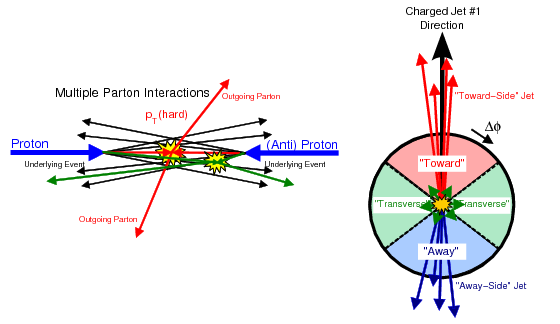
\includegraphics[width=0.8\textwidth]{figures/c3/c3_cms_underlyingevents.png}
 \end{center}
 \caption{Left: Illustration of the underlying event modeled by PYTHIA, togather with hard process. Right: Illustration of the correlations in the azimuthal angle relative to the direction of the leading charged jet}
 \label{fig:c3cmsunderlyingevents}
\end{figure}

In CMS, we use two generators to complete the physics process simulation. First, A multi-purpose parton level generator (e.g. MadGraph\cite{Alwall:2011uj}) will calculate the matrix elements and parton with the PDF input. Then, the parton will be delivered to a hadronic event generator (e.g. PYTHIA\cite{Sjostrand:2014zea} or HERWIG\cite{Bellm:2015jjp}). All the stable and intermediate particles will be stored in the MC sample for study. The stable particles will be passed to detector simulation software. This will be described in the next section. 

\subsubsection{Detector performance simulation}

The 4-vectors of the final state particles are ready for next stage after physics process simulation. Then, we need to know the detector responses for those particles. All the particles and their secondary products from electromagnetic or hadronic showers will be traced and simulated by the first principle in the full simulation. 

The core software for this simulation is GEANT4\cite{Agostinelli:2002hh}. The GEANT4 is a software toolkits that simulate the passage of particles through matter. The detector geometry, in this case, CMS detector geometry\cite{Lefebure:1999wja} is the input of GEANT4. Each subdetector has a geometry input class. The corresponding general GEANT4 geometry class will inherit this class. During the simulation, different particles will call various modules when they pass through the CMS detector system, depending on the type of subdetector. 

However, the CPU time of full simulation is huge due to the complicate CMS geometry and nature of first principle calculation. Therefore, the CMS physicists design a fast simulation method\cite{1742-6596-396-6-062016}. The aim of fast simulation is to reduce the CPU time but keep the event simulation quality in the acceptable level. The simplifications are applied in several parts. For example, the pile-up simulation is simplified, the tracker geometry is roughened, and the showers are simulated with empirical formula rather than first principle. The simulation process has been largely accelerated after those simplifications. 

The fast simulation method is applied on the SUSY signals, and some of the standard model processes. We can use the high level object, like jet, without worries in the fast-simulated samples. However, we need to be careful when we use the higher-level information (e.g. quark-gluon likelihood) in those simplified samples since the geometry are simplified. For example, in this thesis, the customized top tagger needs a fast-full simulation scale factor before the limit setting. We will have more discussion on this in the next chapter. 
